\subsection*{Un incident, puis une année de pertes}

La figure~\ref{fig:lecture-incident} détaille l'exemple du flux annuel : l'incident part de P4,
atteint P1 puis P2 et s'arrête. C'est une marche possible sans choc commun, où P4 est une amorce
ordinaire. Elle compte pour un incident dans l'année, avec un coût $a+b+c$ ; les pertes
élémentaires peuvent être nulles. Dans la variante à perte unique, le même ensemble atteint reçoit
un seul coût tiré : toucher davantage de piliers n'ajoute alors aucun coût. La comparaison au
\S\ref{sec:institut-unite-perte} mesure ce que cette convention change au capital.

\begin{figure}[H]\centering
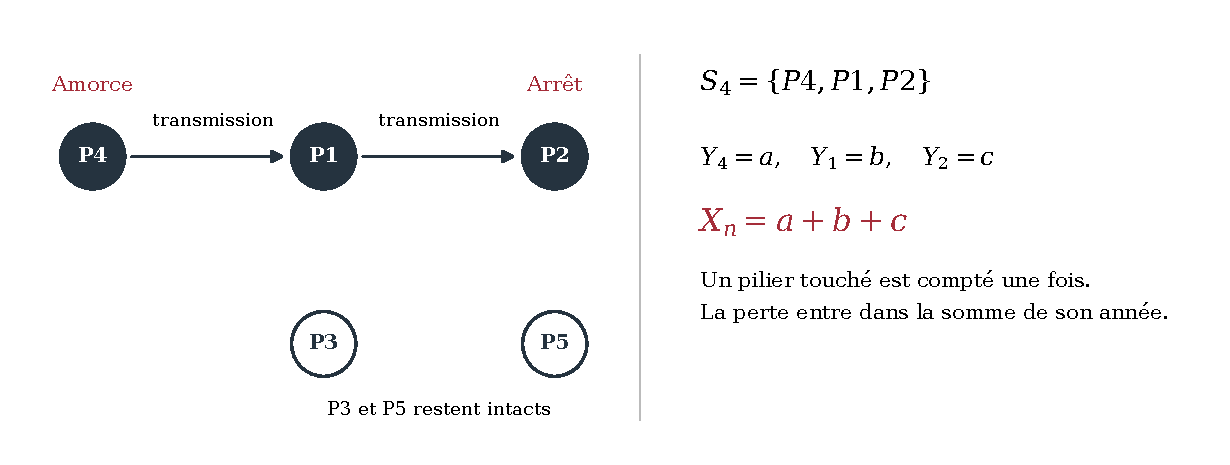
\includegraphics[width=\textwidth]{figures_pedagogie/incident_pas_a_pas.pdf}
\caption{Exemple de lecture, sans calibration nouvelle : une marche P4$\to$P1$\to$P2 donne un ensemble atteint et une perte. Sous le choc commun, P4 peut toucher directement plusieurs autres piliers ; la règle de perte reste additive.}
\label{fig:lecture-incident}
\end{figure}

\begin{table}[H]\centering\small
\renewcommand{\arraystretch}{1.18}
\begin{tabularx}{\textwidth}{@{}p{.16\textwidth}>{\raggedright\arraybackslash}X@{}}
\toprule
\textbf{Étape} & \textbf{Pseudo-code d'une configuration de conformité} \\
\midrule
Préparer & Fixer $(\lambda,p_u,g,\omega)$, les lois de pertes et les probabilités d'amorce ; calculer la loi des ensembles atteints par amorce. \\
Compter & Tirer le nombre $N_y$ d'incidents de chaque année $y$ selon la binomiale négative. \\
Propager & Pour chaque incident, tirer l'amorce puis l'ensemble atteint selon sa loi. Pour P4, appliquer le choc commun si cette configuration le prévoit. \\
Chiffrer & Tirer les pertes élémentaires, masquer les piliers intacts, puis sommer : $X_n=\sum_{k\in S_a}Y_{n,k}$. \\
Agréger & Affecter chaque incident à son année : $L_y=\sum_{n=1}^{N_y}X_n$. \\
Comparer & Calculer le quantile annuel à $99{,}5\,\%$ pour chaque graine, puis comparer les configurations. \\
\bottomrule
\end{tabularx}
\caption{Calcul du scénario à quatre canaux. Le pseudo-code décrit le calcul ; le code tire les sévérités par lots et utilise les lois d'ensembles pré-calculées. Source : \texttt{canaux\_conformite.py}, fonctions \texttt{pertes\_annuelles} et \texttt{metriques\_par\_graine}.}
\label{tab:lecture-algorithme}
\end{table}
